%% LyX 2.3.7 created this file.  For more info, see http://www.lyx.org/.
%% Do not edit unless you really know what you are doing.
\documentclass[english]{beamer}
\usepackage[T1]{fontenc}
\usepackage[latin9]{inputenc}
\setcounter{secnumdepth}{3}
\setcounter{tocdepth}{3}
\usepackage{babel}
\usepackage{graphicx}
\ifx\hypersetup\undefined
  \AtBeginDocument{%
    \hypersetup{unicode=true,pdfusetitle,
 bookmarks=true,bookmarksnumbered=false,bookmarksopen=false,
 breaklinks=false,pdfborder={0 0 1},backref=false,colorlinks=true}
  }
\else
  \hypersetup{unicode=true,pdfusetitle,
 bookmarks=true,bookmarksnumbered=false,bookmarksopen=false,
 breaklinks=false,pdfborder={0 0 1},backref=false,colorlinks=true}
\fi

\makeatletter

%%%%%%%%%%%%%%%%%%%%%%%%%%%%%% LyX specific LaTeX commands.
%% A simple dot to overcome graphicx limitations
\newcommand{\lyxdot}{.}


%%%%%%%%%%%%%%%%%%%%%%%%%%%%%% Textclass specific LaTeX commands.
% this default might be overridden by plain title style
\newcommand\makebeamertitle{\frame{\maketitle}}%
% (ERT) argument for the TOC
\AtBeginDocument{%
  \let\origtableofcontents=\tableofcontents
  \def\tableofcontents{\@ifnextchar[{\origtableofcontents}{\gobbletableofcontents}}
  \def\gobbletableofcontents#1{\origtableofcontents}
}
\newenvironment{lyxcode}
  {\par\begin{list}{}{
    \setlength{\rightmargin}{\leftmargin}
    \setlength{\listparindent}{0pt}% needed for AMS classes
    \raggedright
    \setlength{\itemsep}{0pt}
    \setlength{\parsep}{0pt}
    \normalfont\ttfamily}%
   \def\{{\char`\{}
   \def\}{\char`\}}
   \def\textasciitilde{\char`\~}
   \item[]}
  {\end{list}}

%%%%%%%%%%%%%%%%%%%%%%%%%%%%%% User specified LaTeX commands.
\usetheme[secheader]{Boadilla}
\usecolortheme{seahorse}
\title[FP and declarative programming]{Functional programming and declarative programming}
\author{Sergei Winitzki}
\date{2024-04-14}
\institute[ABTB]{Academy by the Bay 2024}
\setbeamertemplate{headline}{} % disable headline at top
\setbeamertemplate{navigation symbols}{} % disable navigation bar at bottom
\usepackage[all]{xy} % xypic
%\makeatletter
% Macros to assist LyX with XYpic when using scaling.
\newcommand{\xyScaleX}[1]{%
\makeatletter
\xydef@\xymatrixcolsep@{#1}
\makeatother
} % end of \xyScaleX
\makeatletter
\newcommand{\xyScaleY}[1]{%
\makeatletter
\xydef@\xymatrixrowsep@{#1}
\makeatother
} % end of \xyScaleY

% Double-stroked fonts to replace the non-working \mathbb{1}.
\usepackage{bbold}
\DeclareMathAlphabet{\bbnumcustom}{U}{BOONDOX-ds}{m}{n} % Use BOONDOX-ds or bbold.
\newcommand{\custombb}[1]{\bbnumcustom{#1}}
% The LyX document will define a macro \bbnum{#1} that calls \custombb{#1}.

\usepackage{relsize} % make math symbols larger or smaller
\usepackage{stmaryrd} % some extra symbols such as \fatsemi
% Note: using \forwardcompose inside a \text{} will cause a LaTeX error!
\newcommand{\forwardcompose}{\hspace{1.5pt}\ensuremath\mathsmaller{\fatsemi}\hspace{1.5pt}}


% Make underline green.
\definecolor{greenunder}{rgb}{0.1,0.6,0.2}
%\newcommand{\munderline}[1]{{\color{greenunder}\underline{{\color{black}#1}}\color{black}}}
\def\mathunderline#1#2{\color{#1}\underline{{\color{black}#2}}\color{black}}
% The LyX document will define a macro \gunderline{#1} that will use \mathunderline with the color `greenunder`.
%\def\gunderline#1{\mathunderline{greenunder}{#1}} % This is now defined by LyX itself with GUI support.

% Scala syntax highlighting. See https://tex.stackexchange.com/questions/202479/unable-to-define-scala-language-with-listings
%\usepackage[T1]{fontenc}
%\usepackage[utf8]{inputenc}
%\usepackage{beramono}
%\usepackage{listings}
% The listing settings are now supported by LyX in a separate section "Listings".
\usepackage{xcolor}

\definecolor{scalakeyword}{rgb}{0.16,0.07,0.5}
\definecolor{dkgreen}{rgb}{0,0.6,0}
\definecolor{gray}{rgb}{0.5,0.5,0.5}
\definecolor{mauve}{rgb}{0.58,0,0.82}
\definecolor{aqua}{rgb}{0.9,0.96,0.999}
\definecolor{scalatype}{rgb}{0.2,0.3,0.2}
\usepackage[nocenter]{qtree}
\usepackage{relsize}
\renewcommand\arraystretch{1.4}

\makeatother

\usepackage{listings}
\lstset{language=Scala,
morekeywords={{scala}},
otherkeywords={=,=>,<-,<\%,<:,>:,\#,@,:,[,],.,???},
keywordstyle={\color{scalakeyword}},
morekeywords={[2]{String,Short,Int,Long,Char,Boolean,Double,Float,BigDecimal,Seq,Map,Set,List,Option,Either,Future,Vector,Range,IndexedSeq,Try,true,false,None,Some,Left,Right,Nothing,Any,Array,Unit,Iterator,Stream}},
keywordstyle={[2]{\color{scalatype}}},
frame=tb,
aboveskip={1.5mm},
belowskip={0.5mm},
showstringspaces=false,
columns=fullflexible,
keepspaces=true,
basicstyle={\smaller\ttfamily},
extendedchars=true,
numbers=none,
numberstyle={\tiny\color{gray}},
commentstyle={\color{dkgreen}},
stringstyle={\color{mauve}},
frame=single,
framerule={0.0mm},
breaklines=true,
breakatwhitespace=true,
tabsize=3,
framexleftmargin={0.5mm},
framexrightmargin={0.5mm},
xleftmargin={1.5mm},
xrightmargin={1.5mm},
framextopmargin={0.5mm},
framexbottommargin={0.5mm},
fillcolor={\color{aqua}},
rulecolor={\color{aqua}},
rulesepcolor={\color{aqua}},
backgroundcolor={\color{aqua}},
mathescape=false,
extendedchars=true}
\begin{document}
\global\long\def\gunderline#1{\mathunderline{greenunder}{#1}}%
\global\long\def\bef{\forwardcompose}%
\global\long\def\bbnum#1{\custombb{#1}}%
\frame{\titlepage}
\begin{frame}{Outline}

Functional programming is interesting, but in a weird way
\begin{itemize}
\item FP is (almost) engineering
\item Other programming paradigms are (almost) artisanship 
\end{itemize}
A definition of declarative programming:
\begin{itemize}
\item A language for problem requirements, understandable to people
\item The same language is mechanically translated into code
\item The only known ``silver bullet'' of programming
\end{itemize}
Declarative programming must be domain-specific (DSL)
\begin{itemize}
\item We get a productivity boost as long as we avoid the pitfalls
\end{itemize}
Implementing DSLs is a ``killer app'' for functional programming
\begin{itemize}
\item FP is declarative for working with recursive data structures, such
as labeled trees
\item Requires learning some programming language theory
\end{itemize}
\end{frame}

\begin{frame}{Is the Functional Programming community weird?}

The FP community is unlike other programmers' communities
\begin{itemize}
\item Others are focused on a chosen programming language (Java, Python,
JavaScript, etc.), and on designing and using libraries and frameworks
\begin{itemize}
\item \emph{``setup this YAML config, override this method, use this annotation''}
\end{itemize}
\item People in the FP community talk in a very different way
\begin{itemize}
\item \emph{``referential transparency, algebraic data types, monoid laws,
parametric polymorphism, free applicative functors, monad transformers,
Yoneda lemma, Curry-Howard isomorphism, profunctor lenses, catamorphisms''}
\begin{itemize}
\item \href{https://degoes.net/articles/fp-glossary}{A glossary of FP terminology}
(more than $100$ terms)
\end{itemize}
\item From SBTB 2018: \emph{\href{https://www.youtube.com/watch?v=L0aYcq1tqMo}{The Functor,  Applicative,  Monad talk}}
\begin{itemize}
\item By 2018, everyone \emph{expects} to hear these concepts mentioned 
\end{itemize}
\end{itemize}
\end{itemize}
As a former theoretical physicist, I recognize that sort of jargon 
\begin{itemize}
\item The FP jargon is used similarly to an engineer's jargon
\item It is based on math but heavily adapted to the engineering domain
\begin{itemize}
\item Rigor is on the need-to-know basis, mathematical abstraction is limited 
\end{itemize}
\end{itemize}
\end{frame}

\begin{frame}{Programming as engineering vs.~artisanship}

\begin{itemize}
\item FP is similar to engineering in how it uses math-based tools
\begin{itemize}
\item Mechanical, electrical, chemical engineering use calculus, complex
variables, classical and quantum mechanics, electrodynamics, thermodynamics,
physical chemistry
\item FP uses category theory, type theory, logic proof theory, $\lambda$-calculus
\end{itemize}
\item Engineers use \emph{a lot} of special terminology
\begin{itemize}
\item Examples from mechanical, electrical, chemical engineering: \href{https://serc.carleton.edu/NAGTWorkshops/mineralogy/mineral_physics/tensors.html}{rank-4 tensors},
\href{https://mecharithm.com/learning/lesson/holonomic-nonholonomic-constraints-robots-103}{Lagrangians with non-holonomic constraints},
\href{https://www.youtube.com/watch?v=KAbqISZ6SHQ}{Fourier transform of the delta function},
\href{https://ocw.mit.edu/resources/res-6-008-digital-signal-processing-spring-2011/video-lectures/lecture-6-the-inverse-z-transform/}{inverse Z-transform},
\href{https://handbook.uts.edu.au/subjects/41384.html}{Gibbs free energy 1},
\href{https://help.ebsilon.com/EN/Component_134.html}{2}
\item Examples from FP: \href{https://wiki.haskell.org/Rank-N_types}{rank-$N$ types},
\href{https://www.cs.toronto.edu/~lczhang/324/ex/a2.pdf}{continuation-passing transformation},
\href{https://stackoverflow.com/questions/20152939/what-is-a-polymorphic-lambda}{polymorphic lambda functions},
\href{https://stackoverflow.com/questions/13352205/what-are-free-monads}{free monads},
\href{https://stackoverflow.com/questions/49135351/deforestation-in-a-hylomorphism}{hylomorphisms}
\end{itemize}
\item As in engineering, the special terminology in FP is \emph{not} self-explanatory
\begin{itemize}
\item ``Gibbs free energy'' is not energy that \href{https://de.wikipedia.org/wiki/Josiah_Willard_Gibbs}{J.�W.�Gibbs}
provides for free
\end{itemize}
\end{itemize}
All that stuff is mathematics-based knowledge that needs learning
\begin{itemize}
\item Programmers today neither study as engineers, nor work as engineers
\end{itemize}
\end{frame}

\begin{frame}{Books on engineering vs.~artisanship}

Functional programming looks like engineering

Today's ``software engineering'' resembles artisanship
\begin{center}
\vspace{-0.3\baselineskip}
Books on mechanical, electrical, chemical engineering design:
\par\end{center}

\begin{center}
\includegraphics[width=0.2\columnwidth]{\string"Jazar. Theory of Applied Robotics 2nd edition - sample page\string".png}\includegraphics[width=0.2\columnwidth]{\string"Schaum's outline of electric curcuits, 4th edition - sample page\string".png}\includegraphics[width=0.2\columnwidth]{\string"Ellingson - Electromagnetics vol. 2, sample page\string".png}\includegraphics[width=0.2\columnwidth]{\string"Sinnott, Tower. Chemical Engineering Design 5th edition - sample page\string".png}\vspace{-0.3\baselineskip}
\par\end{center}

\begin{center}
Books on software design and architecture:\vspace{-0.3\baselineskip}
\par\end{center}

\begin{center}
\includegraphics[width=0.2\columnwidth]{\string"Solid software design architecture handbook - sample page\string".png}\includegraphics[width=0.16\columnwidth]{\string"Clean architecture - sample page\string".png}\includegraphics[width=0.14\columnwidth]{\string"Code Complete - sample page\string".png}\includegraphics[width=0.2\columnwidth]{\string"Code Complete - another sample page\string".png}
\par\end{center}

\end{frame}

\begin{frame}{Questions that have rigorous answers}

In engineering, certain questions about device design have rigorous
answers

In FP, certain questions about code design have rigorous answers
\begin{itemize}
\item The answers are \emph{not} a matter of opinion or experience
\item The answers are found via mathematical derivations and reasoning
\item The answers guide the design
\end{itemize}
Examples of reasoning tasks:
\begin{itemize}
\item Can we implement these APIs?
\end{itemize}
\begin{lyxcode}
\textcolor{blue}{\footnotesize{}f~::~(r~->~Either~z~a)~->~Either~z~(r~->~a)~-{}-~Haskell}{\footnotesize\par}

\textcolor{blue}{\footnotesize{}g~::~Either~z~(r~->~a)~->~r~->~Either~z~a}{\footnotesize\par}

\textcolor{blue}{\footnotesize{}def~f{[}Z,~R,~A{]}(r:~R~=>~Either{[}Z,~A{]}):~Either{[}Z,~R~=>~A{]}~//~Scala}{\footnotesize\par}

\textcolor{blue}{\footnotesize{}def~g{[}Z,~R,~A{]}(e:~Either{[}Z,~R~=>~A{]}):~R~=>~Either{[}Z,~A{]}}{\footnotesize\par}
\end{lyxcode}
\begin{itemize}
\item Can use the data structure \texttt{\textcolor{blue}{\footnotesize{}F}}
as a monad in our code?
\end{itemize}
\begin{lyxcode}
\textcolor{blue}{\footnotesize{}type~F~a~=~Maybe~(a,~a,~a)~-{}-~Haskell}{\footnotesize\par}

\textcolor{blue}{\footnotesize{}bind~::~F~a~->~(a~->~F~b)~->~F~b}{\footnotesize\par}

\textcolor{blue}{\footnotesize{}type~F{[}A{]}~=~Option{[}(A,~A,~A){]}~//~Scala}{\footnotesize\par}

\textcolor{blue}{\footnotesize{}def~flatMap{[}A,~B{]}(fa:~F{[}A{]})(f:~A~=>~F{[}B{]}):~F{[}B{]}}{\footnotesize\par}
\end{lyxcode}
\end{frame}

\begin{frame}{A definition of ``declarative''}

Programming is ``declarative'' when \emph{``specifications} \emph{are}
\emph{programs''}
\begin{itemize}
\item ``Being declarative'' is not a property of a programming language
alone
\end{itemize}
A language $L$ is \textbf{declarative for an application domain}
$D$ if: 
\begin{itemize}
\item The domain $D$ has a good specification formalism $F$ 

\begin{itemize}
\item ``good'' = visual, pragmatically convenient, complete for the domain
$D$ 
\end{itemize}
\item There is a syntactic translation from $F$ to $L$
\item The resulting program correctly implements the specification
\end{itemize}
Less formally:
\begin{itemize}
\item A declarative language is a ``readable DSL'' for the given domain
\end{itemize}
\end{frame}

\begin{frame}{Example: declarative FORTRAN 77}

\begin{itemize}
\item Application domain: numerical mathematical expressions
\item Specification: a mathematical formula involving \emph{numbers }and\emph{
functions}
\item Example specification: 
\[
f(x,p,q)=\frac{\sin px}{x^{2}}-\frac{(\sin qx)^{2}}{x^{3}}
\]

\begin{itemize}
\item Implementation: \texttt{\textcolor{blue}{F(X,P,Q) = SIN(P{*}X)/X{*}{*}2-(SIN(Q{*}X)){*}{*}2/X{*}{*}3}}
\end{itemize}
\item For more complicated tasks, FORTRAN is not declarative
\[
\tilde{X}_{k}=Y_{k}-\sum_{j=k+1}^{n}A_{kj}X_{j},\quad\forall k\in\left[1..n\right]
\]
\end{itemize}
\begin{center}
\includegraphics[width=0.4\textwidth]{../../talks/prolog/fortran1}$\quad$(example
code, 1987)
\par\end{center}

\end{frame}

\begin{frame}{Example: declarative Haskell 98}

\begin{itemize}
\item Application domain: recursively defined, algebraic data structures
\item Specifications: inductive definitions of functions on ADTs
\item Example (from R. Sedgewick, \emph{Algorithms in C}, 1998)
\end{itemize}
\begin{center}
\includegraphics[width=1\textwidth]{../../talks/prolog/sedgewick-alg-tree}
\par\end{center}

\texttt{\textcolor{blue}{data BTree $\alpha$ = BTNode $\alpha$ |
BTVertex $\alpha$ (BTree $\alpha$) (BTree $\alpha$)}}

\texttt{\textcolor{blue}{~}}\textcolor{blue}{{} }

\texttt{\textcolor{blue}{enum BTree{[}+A{]}: ~ ~ //Scala}}

\texttt{\textcolor{blue}{~ case BTNode{[}A{]}(a: A)}}

\texttt{\textcolor{blue}{~ case BTVertex{[}A{]}(a: A, left: BTree{[}A{]},
right: BTree{[}A{]})}}
\end{frame}

\begin{frame}{Example: declarative Haskell 98, continued}

\begin{center}
\includegraphics[width=1\textwidth]{../../talks/prolog/sedgewick-fun-tree}
\par\end{center}

\texttt{\textcolor{blue}{height :: BTree $\alpha$ $\rightarrow$
Int~ ~ -{}- Haskell}}

\texttt{\textcolor{blue}{height (BTNode \_) = 0}}

\texttt{\textcolor{blue}{height (BTVertex \_ t1 t2) = 1 + max (height
t1) (height t2)}}

\texttt{\textcolor{blue}{~}}

\texttt{\textcolor{blue}{def height{[}A{]}: BTree{[}A{]} => Int =
\{ ~ ~ //Scala}}

\texttt{\textcolor{blue}{~ ~ case BTNode(\_) => 0}}

\texttt{\textcolor{blue}{~ ~ case BTVertex(\_, t1, t2) =>}}

\texttt{\textcolor{blue}{~ ~ ~ 1 + math.max(height(t1), height(t2))}}

\texttt{\textcolor{blue}{\}}}
\end{frame}

\begin{frame}{Example: non-declarative Haskell}

For a different application domain, Haskell is \emph{not} declarative!
\begin{itemize}
\item Downloading data from server (from ``\emph{Real World Haskell}'',
2008)
\end{itemize}
\begin{center}
\includegraphics[width=1\textwidth]{../../talks/prolog/haskell-ugly-download}
\par\end{center}

\end{frame}

\begin{frame}{Declarative programming: Stories of success}

Success stories (achieved the goals of declarative programming)
\begin{itemize}
\item Infix arithmetic: numerical math
\item SQL: relational queries
\item Autolayout: GUI layout on iOS and MacOS
\item Haskell, Scala: Parsing, type-checking, evaluation of DSLs
\item Prolog: logic puzzles (next slide)
\begin{itemize}
\item for comparison, see: \href{https://stackoverflow.com/questions/34206275/matrix-multiplication-with-prolog}{Matrix multplication with Prolog}
\end{itemize}
\item \href{https://www.classes.cs.uchicago.edu/archive/2007/spring/32102-1/papers/p372-fournet.pdf}{Chemical Abstract Machine}:
\href{https://rosettacode.org/wiki/Dining_philosophers\#JoCaml}{dining philosophers problem}
\end{itemize}
\end{frame}

\begin{frame}{Prolog as a DSL for logic puzzles}

\textcolor{teal}{All jumping creatures are green. All small jumping
creatures are martians. All green martians are intelligent. Ngtrks
is small and green. Pgvdrk is a jumping martian. Who is intelligent?}
{\footnotesize{}(inpired by }\emph{\footnotesize{}\href{https://isfdb.org/cgi-bin/title.cgi?1392619}{Invasion from Aldebaran}}{\footnotesize{})}\\

\begin{lyxcode}
\$~cat~>~martians.pl

\textcolor{blue}{green(X)~:-~jumping(X).}

\textcolor{blue}{martian(X)~:-~small(X),~jumping(X).~}

\textcolor{blue}{intelligent(X)~:-~green(X),~martian(X).}

\textcolor{blue}{small(ngtrks).~green(ngtrks).}

\textcolor{blue}{jumping(pgvdrk).~martian(pgvdrk).}

\textcolor{blue}{question~:-~}

\textcolor{blue}{{}~~intelligent(X),~format('\textasciitilde w~is~intelligent.\textasciitilde n',~X),~halt.}~\\

\textasciicircum D~

\$~brew~install~swi-prolog

\$~swipl~-o~martians~-q~-t~question~-c~martians.pl

\$~./martians~

pgvdrk~is~intelligent.
\end{lyxcode}
\end{frame}

\begin{frame}{Declarative programming: Pitfalls}

When does declarative programming fail:
\begin{itemize}
\item Declarative language is used outside its domain
\item Specifications become too large to understand
\begin{itemize}
\item Make specifications modular and understandable in isolation
\begin{itemize}
\item Example: domain-specific notations in mathematical sciences
\end{itemize}
\item Make DSL languages and programs small, and keep them small
\end{itemize}
\end{itemize}
Signs that programming becomes non-declarative:
\begin{itemize}
\item Lots of code has no clear mapping to the problem domain
\begin{itemize}
\item Example: ``dining philosophers'' \href{https://rosettacode.org/wiki/Dining_philosophers}{in most programming languages}
\end{itemize}
\item Code appears to say one thing but does another thing when run
\begin{itemize}
\item ``To shutdown the computer, press the \textbf{Start} button''
\item Leaky abstractions. What does \texttt{\textcolor{blue}{f()}} return?
\end{itemize}
\begin{lyxcode}
\textcolor{blue}{var~x~=~0;~~~~//~JavaScript}

\textcolor{blue}{function~f()~\{~return~x;~\}~//~Returns~zero?}

\textcolor{blue}{//~But~what~if~another~module~does~this:}

\textcolor{blue}{var~y~=~f();~y~=~\textquotedbl abc\textquotedbl ;}
\end{lyxcode}
\end{itemize}
\end{frame}

\begin{frame}{Declarative programming: Stories of failure}

Failure stories (did not turn out to be declarative)
\begin{itemize}
\item Programming languages resembling English (\href{https://techdocs.broadcom.com/us/en/ca-mainframe-software/database-management/ca-idms-reference/19-0/callable-services-reference/tcp-ip-api-support/tcp-ip-programming-examples/cobol-examples.html}{COBOL},
\href{https://github.com/kevin-funderburg/AppleScripts/blob/master/Script-Development/Click-at-Mouse-Location.applescript}{AppleScript})
\begin{itemize}
\item Programs become long and unreadable
\end{itemize}
\item Languages where everything is a built-in feature (\href{https://techdocs.broadcom.com/us/en/ca-mainframe-software/database-management/ca-idms-reference/19-0/callable-services-reference/tcp-ip-api-support/tcp-ip-programming-examples/pl-i-examples.html}{PL/I},
\href{https://github.com/dustinkredmond/abap-examples/blob/main/Z_SIMPLE_ALV_GRID.abap}{ABAP})
\begin{itemize}
\item Features interact in unforeseen ways, corner cases lead to bugs
\end{itemize}
\item ``Mark-up'' languages (XML, HTML)
\begin{itemize}
\item Used mostly outside their domain of declarativeness
\end{itemize}
\end{itemize}
\end{frame}

\begin{frame}{Failures of XML and HTML}

Failed due to predominant usage \emph{outside} their designated domain

Intended usage (SGML, XML, HTML): plain text with occasional mark-up

\vspace{-1\baselineskip}

\begin{lyxcode}
\textcolor{blue}{<p>~Hello!~This~is~the~home~page~of~John~Doe,~a~graduate}

\textcolor{blue}{student~at~the~Department~of~Electrical~Engineering~and}

\textcolor{blue}{Computer~Science,~University~of~California,~Los~Angeles.}

\textcolor{blue}{<p>~You~can~click~<a~href=\textquotedbl cv.html\textquotedbl >here</a>~to~read}

\textcolor{blue}{my~CV.~This~page~is~under~construction!~Good~bye!}
\end{lyxcode}
In real life:
\begin{itemize}
\item XML: used as a data representation language (SOAP, config files)
\item HTML: used as a GUI layout language for the Web
\end{itemize}
\begin{center}
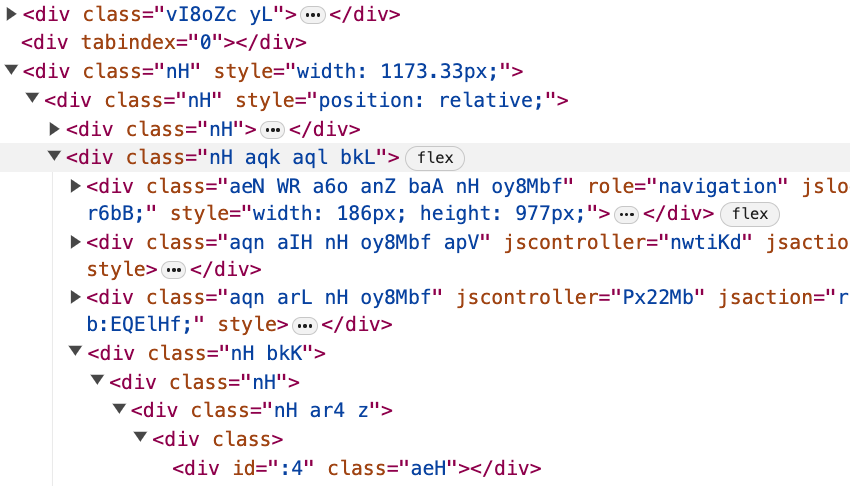
\includegraphics[width=0.3\paperwidth]{modern-html}
\par\end{center}

\end{frame}

\begin{frame}{The joy of implementing DSLs in FP languages}

Two choices for implementing a DSL:
\begin{itemize}
\item Embedded DSL
\item External DSL
\end{itemize}
In both cases, FP works great
\begin{itemize}
\item For embedded DSLs:
\begin{itemize}
\item Free monads, GADTs, non-leaky abstractions, strict typing
\end{itemize}
\item For external DSLs:
\begin{itemize}
\item Parser combinators, recursion schemes, GADTs, HOAS / PHOAS
\end{itemize}
\end{itemize}
Anecdotal evidence: one-person languages with compilers in Haskell
\begin{itemize}
\item \href{https://wiki.portal.chalmers.se/agda/pmwiki.php}{Agda} (Ulf
Norell, 2007)
\item \href{https://www.idris-lang.org/}{Idris} (Edwin Brady, 2007)
\item \href{https://elm-lang.org/}{Elm} (Evan Czaplicki, 2012)
\item \href{https://www.purescript.org/}{PureScript} (Phil Freeman, 2013)
\item \href{https://dhall-lang.org/}{Dhall} (Gabriella Gonzalez, 2016)
\begin{itemize}
\item Time to re-implement Dhall in Scala: 2 months, 4K LOC
\end{itemize}
\end{itemize}

\end{frame}

\begin{frame}{Conclusions}

Functional programming has a steep learning curve
\begin{itemize}
\item Using FP techniques makes programmers' work closer to \emph{engineering}
\item Most artisans don't want to become engineers 
\end{itemize}
Declarative programming means a symbiosis between human tradition
and formal mathematics
\begin{itemize}
\item Best implemented by math-based programming paradigms
\begin{itemize}
\item FP and logic programming
\end{itemize}
\end{itemize}
Implementing DSLs is one of FP's ``killer apps''
\begin{itemize}
\item Even a small DSL is a productivity boost when it is declarative for
the chosen domain
\item FP languages are \href{https://github.com/dhall-lang/dhall-lang/blob/master/standard/beta-normalization.md}{simple to implement}
once you get the theory
\end{itemize}
\end{frame}

\end{document}
